\chapter{Machine learning for GPS clock prediction}


%====================================================================================================
\section{GPS clock adjusment}

%----------------------------------------------------------------------------------------------------
\subsection{Satellite and reference clocks}

%----------------------------------------------------------------------------------------------------
\subsection{Satellite brodcasted polynomial}
Currently every GPS device is able to calculate satellite clock bias based on
%TODO: Algorithm is configuring not message
parameters broadcasted in navigation message by the satellite itself which 
configure a second-degree polynomial:
\begin{equation}
	\Delta t_{sv}=a_{f0}+a_{f1}(t-t_{ref})+a_{f2}(t-t_{ref})^2+\Delta t,
\end{equation}
where $a_{f0}$, $a_{f1}$ and $a_{f2}$ are parameters sent in a satellite message, $t$ is GPS
time and $t_{ref}$ is a reference time. 
$\Delta t$ is the periodical component of a relativistic correction which is caused by 
gravitational field of earth and by a speed at which satellite orbits the planet.
This component is dependent on the orbit eccentricity and can be described as a:
\begin{equation}
 \Delta t=- 2\, \frac{\mathbf{r}_s \cdot \mathbf{v}_s}{c^2} \qquad,
\end{equation}
where $ {\mathbf r}_s$ and ${\mathbf v}_s$ are the satellite 
%TODO: Write more eloquently about units.
position ($\displaystyle m$) and velocity ($\displaystyle m/s$) vectors in an inertial system. 
While this method allows real-time corrections its precision is at the range of
nanoseconds \cite{Misra2011}, which results in an error of about 30 cm in localization calculation.
While this may be acceptable in-car navigation, robotic solutions require more precision that in
turn requires clock correction on the level of picoseconds.
Such corrections used along with proper measurement processing algorithm,
like Precise Point Positioning algorithm (PPP), will allow real-time or quasi-real-time localization with 
precision in the range of single centimeters\cite{krzan2015}.

%----------------------------------------------------------------------------------------------------
\subsection{IGU products}
The most widely used source of precise clock corrections are products provided 
by International GNSS Service (IGS) \cite{IGS}.
% TODO:Fix table size so it is not wider than text
\begin{table}[ht] 
	\centering
	\caption{Variants of IGS products}
	\label{tab:igs_products}
	\begin{tabular*}{\textwidth}{*{5}{l}}
		\hline
		\hline
		Type& Accuracy& Latency& Update& Sample \\
		&&&&interval\\
		\hline
		Transmitted & 5ns & real time & -- & daily  \\
		Ultra rapid -- predicted & 3ns & real time & at 03, 09, 15, 21 UTC & 15 min  \\
		Ultra rapid -- observed & 150ps & 3-9 hours & at 03, 09, 15, 21 UTC & 15 min  \\
		Rapid & 75ps & 17-41 hours & at 17 UTC daily & 5 min \\
		Final & 75ps & 12-18 days & every Thursday & 30 s \\
		\hline
		\hline
	\end{tabular*}
\end{table}
Values shown in Table \ref{tab:igs_products} refer to satellite clock bias only,  IGS products
provide other information which full description  is available at  
\texttt{http://www.igs.org/products}.
IGS products can be easily divided into two categories:
\begin{itemize}
	\item real time consisting of transmitted and ultra rapid predicted half,
	\item high latency consisting of ultra rapid observed half as well as rapid and final products.
\end{itemize}
Solutions that have high latency are not usable in real-time navigation and as such will not be
considered in this work. Ultra-rapid observed part will be used as a source of
reference time so that if a bias prediction error is equal to zero it means that is
the same as provided by Ultra-rapid observed.
As can be seen in the Table \ref{tab:igs_products} all real-time solutions provide precision 
at a range of nanoseconds, aim of this work is to show that LSTM networks can provide 
better results than those solutions while still working at real-time response latency.

%====================================================================================================
\section{Classic ML approaches}

%----------------------------------------------------------------------------------------------------
\subsection{Polynomial regression}

%----------------------------------------------------------------------------------------------------
\subsection{Frequency analysis and reconstruction}


%====================================================================================================
\section{LSTM neural nerworks}

%----------------------------------------------------------------------------------------------------
\subsection{Research overwiev}
\subsubsection{Machine learning pipeline}
In the project, a machine learning pipeline as described in Figure \ref{fig:pipeline} was used.
\begin{figure}[ht] 
	\centering
	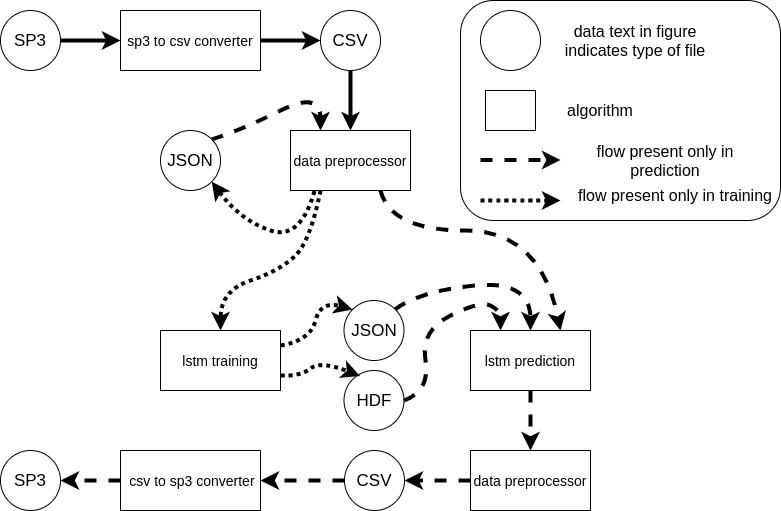
\includegraphics[width=\textwidth]{figures/pipeline}
	\caption{Machine learning pipeline}
	\label{fig:pipeline}
\end{figure}
Data is received in Standard Product 3 (sp3) format that contains information about satellites
orbits as well as about their clocks.
As this is a specialized file format and is not most convenient to work with first step extracts
data from sp3 format into CSV which is a more general-purpose format.
For the next step Python script reads CSV file and stabilizes time series by differentiating it,
this is an important step as neural networks work best with stable data.
The original value of the first element in the series must be stored separately for the recreation
of the original data format. In the next step, stable data is shifted so that its median 
is at zero.
The last step that is common for all data pipelines is scaling, for best predictions in neural
networks, a value from the range of $[-1 , 1]$ should be used. While it is not possible 
to assure that no future data will fit into that range it is possible to make it less likely.
%TODO: Write more precisely how we deal with out of range values
The scale is given as an algorithm parameter and may be calculated either based on the clock model
or available data. In the case of this experiment, the largest absolute value in the test set was
used as a scaling factor.
At this moment depending on either this is a train or a prediction pipeline one of two things
will happen.
In the case of the training pipeline, data will be divided into training and evaluation
portions and the neural network will be adjusted to it. The result of this pipeline are *.hdf5 and
*.json files that store respectively weights and topology of a network.
In the case of a prediction pipeline, an already prepared weights and topology will be loaded and
series will be extended with predictions. The number of predictions depends on the prediction depth
parameter. After that time series will be returned to its original form by reverse scaling
median shift and integration.
The predicted part will be returned as a CSV file with epochs starting at the point 
in which the original data ended.
The resulting CSV can be finally converted back into an sp3 file that may be used 
for calibration of localization algorithm.

\subsubsection{Data source}
For this work three of IGS provided products are used. Ultra-rapid observed is used as a
training and network input in the prediction phase. Predicted half of the same product 
is used to compare the prediction quality of LSTM.
The observed half is used as a reference bias, in other words, the bias prediction error is
the difference between the predicted value and IGU observed half.
\begin{table}[ht] \label{table:2}
	\parindent0pt
	\caption{Products used in experiments}
	\centering
	\begin{tabular}{lcl}
		\hline
		\hline
		Type &Accuracy &Latency\\  
		\hline 
		Ultra-Rapid predicted half &1.4 ns &real time\\  
		Ultra-Rapid observed half &50 ps & 3-9 hours\\  
		\hline 
		\hline
	\end{tabular}
\end{table}
This data was downloaded from repositiory provided by European Space Agency\cite{ESA}
It is important to remember that the prediction system designed in this work does not intend to 
compete with long latency high accuracy products but only with those that provide 
real-time predictions.
To test the validity of LSTM as a predictor single satellite (G05) will be used.

\subsubsection{Data preprocessing}
%TODO: Fix next sentence to make it more clear
IGU provides raw clock bias, this poseses two problems for the approach used in this work.
Constant clock drift is a major source of an error it suppresses other error types
as seen in figure \ref{fig:raw_bias} in visualization it makes data seams linear.
\begin{figure}[ht] 
	\centering
	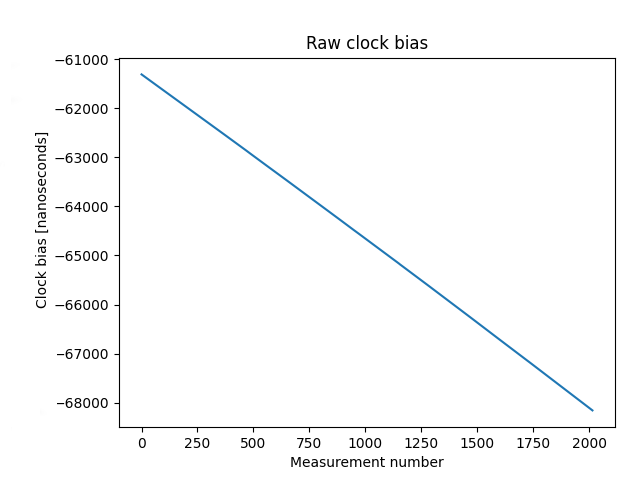
\includegraphics[width=10cm]{figures/bias_raw}
	\caption{Raw clock bias}
	\label{fig:raw_bias}
\end{figure}
This trend implies the non-stationary nature of series, this is a problem as neural networks work 
best for stationary data with mean at 0 and values inbetween -1 and 1.
To solve this problems first series is differentiated which returns data where other noises 
besides constant shift are visible as seen in Figure \ref{fig:diffed_bias}.
\begin{figure}[ht] 
	\centering
	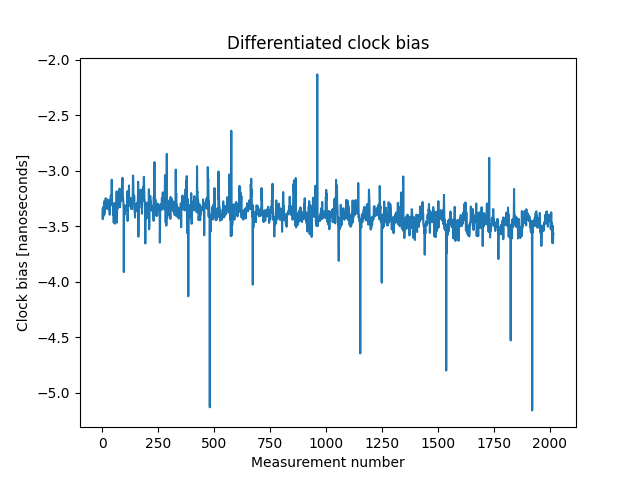
\includegraphics[width=10cm]{figures/bias_diffed}
	\caption{Differentiated clock bias}
	\label{fig:diffed_bias}
\end{figure}
Constant drift is still present as a shift at the y-axis, to remove it a mean 
shift must be performed.
Finally, data must be scaled so that there will be no values with an absolute value above one.
It is, of course, possible for future prediction inputs to have absolute value above one 
however this will not be a problem as the network can deal with such inputs especially 
if they appear rarely in series.
Results of complete preprocessing of signal are visualised in Figure \ref{fig:bias_normalized}
\begin{figure}[ht] 
	\centering
	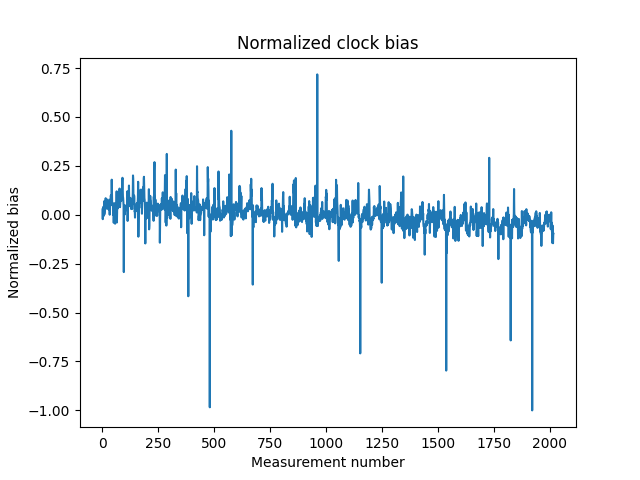
\includegraphics[width=10cm]{figures/bias_normalized}
	\caption{Comparison of differentiated clock bias}
	\label{fig:bias_normalized}
\end{figure}
%----------------------------------------------------------------------------------------------------
\subsection{Phase 1 validation of approach}

\subsubsection{Network configuration and experiments}
For the research a topology with two hidden LSTM layers and a single dense layer as output was 
used as shown on figure \ref{fig:topology}.
Most of the parameters as well as a general topology were set up based on suggestions from 
\cite{Chollet2018}. As an activation function of LSTM layers a rectifier (RELU),
%TODO: What the fuck is tangensoidal ?
tangensoidal as well as sigmoidal function was used.
For dense (output) only a linear activation was used so that there are no limits on predicted 
value.
Mean squared error (MSE), mean average error (MAE) and root mean square (RMS)
was used as a loss function.
Two optimizers will be tested, Root Mean Square Propagation (RMSprop)\cite{Hinton2012} and 
Adaptive Momentum Estimation (Adam)\cite{Kingma2015}.
\begin{figure}[ht] 
	\centering
	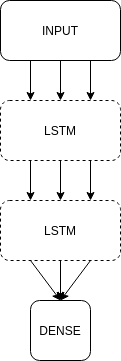
\includegraphics[width=3cm]{figures/topology}
	\caption{Neural Network topology}
	\label{fig:topology}
\end{figure}

As the network learning process is stochastic by nature 10 experiments were run for each
configuration and then average results were compared.
When comparing results RMSProp proven to be a better optimizer, as shown in Table 
\ref{tab:optimizers} and so it was used in the following experiments.
All experiments were run on a dataset obtained on 22.07.2018.
\begin{table}[ht] 
	\centering
	\caption{Optimizers and loss functions}
	\label{tab:optimizers}
	\begin{tabular}{l*{6}{c}}
		\hline
		\hline
		Parameter& \multicolumn{6}{c}{Optimizer}  \\
		&\multicolumn{3}{c}{Adam}&\multicolumn{3}{c}{RMSProp}\\
		\hline
		& MAE & MSE & RMS & MAE & MSE & RMS  \\
		Avarage & 1.10 & 1.38 & 1.15 & 0.80 & 0.79 & 0.87  \\
		$\sigma$ & 0.23 & 0.57 & 0.23 & 0.19 & 0.27 & 0.16  \\
		Min & 0.82 & 0.78 & 0.89 & 0.48 & 0.37 & 0.61  \\
		Max & 1.55 & 2.63 & 1.62 & 0.99 & 1.08 & 1.04  \\
		\hline
		\hline
	\end{tabular}
\end{table}
Repeatability of results was much better in Adam optimizer however that was only due 
to the tendency of this algorithm to stuck in the same local minimum every time it was run.

For the next experiment, three possible activation functions for hidden layers were 
tested with RMSProp as an optimizer. 
In each case, both hidden layers had the same activation function, and the dense layer 
that served as output had linear activation.
\begin{figure}[ht] 
	\centering
	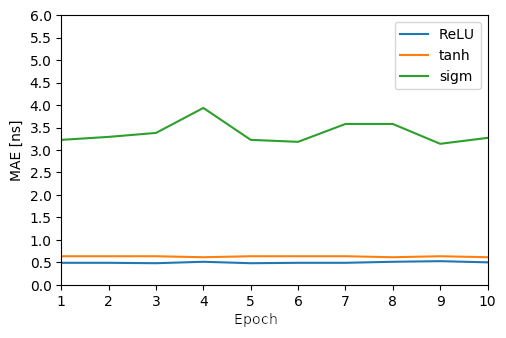
\includegraphics[width=10cm]{figures/activation_to_error}
	\caption{Activation function effect on prediction error}
	\label{fig:activation_to_error}
\end{figure}
As it is seen in Figure \ref{fig:activation_to_error} RELU activation yields the best results,
this was the expected outcome as it is a function commonly used with LSTM layers.
Slightly surprising was the rather good result of tanh that yielded results much closer
to Relu than to sigmoid.
For the following experiments, only Relu was used as a hidden layer activation.
In the next experiment a value of loopback was adjusted, its initial value for previous experiments
was set to 12 as an educated guess.
\begin{table}[ht] 
	\centering
	\caption{Loopback values}
	\label{tab:loopback}
	\begin{tabular}{l*{6}{c}}
		\hline
		\hline
		Parameter& \multicolumn{6}{c}{Loopback}  \\
		& 1& 4& 12& 32& 64& 96\\
		\hline
		Avarage & 0.48 & 0.48 & 0.51 & 0.47 & 0.55 & 0.50  \\
		$\sigma$ & 0.01 & 0.01 & 0.03 & 0.01 & 0.02 & 0.02  \\
		min & 0.47 & 0.46 & 0.47 & 0.46 & 0.52 & 0.47  \\
		max & 0.51 & 0.49 & 0.55 & 0.48 & 0.59 & 0.54  \\
		\hline
		\hline
	\end{tabular}
\end{table}
As can be seen in Table \ref{tab:loopback} the best result was achieved for a loopback value of 32.
Finally, a comparison between Adam and RMSProp was made again with all other parameters 
set according to previous experimental results.
\begin{table}[ht] 
	\centering
	\caption{Optimizers and loss functions for adjusted parameters}
	\label{tab:optimizers2}
	\begin{tabular}{l*{6}{c}}
		\hline
		\hline
		Parameter& \multicolumn{6}{c}{Optimizer}  \\
		&\multicolumn{3}{c}{Adam}&\multicolumn{3}{c}{RMSProp}\\
		\hline
		& MAE & MSE & RMS & MAE & MSE & RMS  \\
		Avarage & 0.87 & 0.95 & 0.94 & 0.66 & 0.63 & 0.76  \\
		$\sigma$ & 0.29 & 0.56 & 0.28 & 0.23 & 0.43 & 0.24  \\
		min & 0.44 & 0.30 & 0.55 & 0.43 & 0.29 & 0.54  \\
		max & 1.38 & 2.06 & 1.43 & 1.12 & 1.71 & 1.31  \\
		\hline
		\hline
	\end{tabular}
\end{table}
When using adjusted parameters average errors become better for all configurations and
results of RMSProp become less consistent due to the higher value of divergence.
However, RMSProp is still an overall better solution than Adam and so it will be used in final
configuration.

After running the experiments and comparing results a final set of network parameters was set
as described in a Table \ref{tab:final_config}.
\begin{table}[ht] 
	\centering
	\caption{Basic network configuration}
	\label{tab:final_config}
	\begin{tabular}{lcc}
		\hline
		\hline
		Parameter& \multicolumn{2}{c}{Hidden layer}  \\
		&First&Second\\
		\hline
		Neuron count & 32 & 128  \\
		Activation function & ReLU & ReLU  \\
		Dropoff & 0.2 & 0.5   \\
		Recurrent dropoff & 0.2 & 0.5   \\
		Regularization & L2 & L2   \\
		Statefullness & NO & NO   \\
		\hline
		\hline
	\end{tabular}
\end{table}


\subsubsection{Comparition with other solutions}
After preparing optimal coniguration of prediction network it predictions were compared agains
linear approximation, polynomial approximation of 2, 4 and 8 degrees as well as against IGU rapid
product predicted half.
As difference between results of polynomial approximation were relatively unsignificant between
polynomials of different degrees all their results will be presented as one rounded to
two decimal points.
\begin{table}[ht] 
	\centering
	\caption{Prediction errors for 24h range}
	\label{tab:comparition_1}
	\begin{tabular}{lccc}
		\hline
		\hline
		Algorithm& \multicolumn{3}{c}{Error value}  \\
		& MAE& MSE& RMS\\
		\hline
		LSTM& 0.47& 0.36& 0.60  \\
		IGU-predicted& 1.60& 2.76& 1.66  \\
		Linear& 1.73& 3.21& 1.79  \\
		Polynomial& 1.33& 1.87& 1.37  \\
		\hline
		\hline
	\end{tabular}
\end{table}
As seen in Table \ref{tab:comparition_1} LSTM network yielded significantly better results than
IGU predicted. What is interesting observation is that polynomial approximation appears to work
better than IGU for 24 hours prediction period.
Next comparison was based on shorter prediction time and as seen in Table \ref{tab:comparition_2}
LSTM gains more advantage over IGU predicted the longer prediction range is.
What more interesting is that LSTM errors actually drop over time.
\begin{table}[ht] 
	\centering
	\caption{Prediction errors for 24h range}
	\label{tab:comparition_2}
	\begin{tabular}{lccc}
		\hline
		\hline
		Algorithm& \multicolumn{3}{c}{RMS for prediction range}  \\
		& 6h& 12h& 24h\\
		\hline
		LSTM& 1.02& 0.76& 0.60  \\
		IGU-predicted& 1.26& 1.31& 1.66  \\
		\hline
		\hline
	\end{tabular}
\end{table}

LSTM predictions were of higher accuracy than linear and polynomial as well as IGU Rapid
predicted which is recognized as a state of the art.


\subsubsection{Conclusions}
In this paper, it was proven that even the with most generic architecture LSTM neural networks are
capable of predicting a bias of the GPS satellite atomic clocks.
It was demonstrated that proposed approach provides better results then IGU predicted 
that is considered as a state of the art in low latency GPS satellite clock bias prediction.

This is good starting point for the future research that should focus on tuning network model for
even better precision of results as well as capability of generalizaion over all active GPS 
satellites.

Adjustment of following elements of network architecture should be considered in future research:
\begin{itemize}
	\item modification of hidden layer size,
	\item application of alternative activation functions like Exponential Linear Unit (ELU)
		or wavelet based activation,
	\item inclusion of additional data from sp3 products as a prediction input,
	\item removal of relativistic correction during preprocessing stage,
	\item removal of outliers from time series.
\end{itemize}

Next step in this research will focus mainly on data preprocessing  as well as on 
application of algorithm in low power devices.

%----------------------------------------------------------------------------------------------------
\subsection{Phase 2 implementation for all satellites}
\subsubsection{Experiment scope}
While initial tests were done only on a single satellite in this phase scope of experiment
was extended to cover most of active GPS satellites.
Satellites launched as a part of GPS system can be divided into a following generations:
\begin{itemize}
	\item original (II)
	\item IIA
	\item IIR
	\item IIR-M
	\item IIF
\end{itemize}
Because all satellites from original group II were retired before 2007 none of them will be 
included in this work. Last satellite from group IIA was retired in september of 2019 and its
data from before that time will be used in this phase.
This results in total of 31 sattelites analyzed from which most use a onboard rubidium clock
ensemble as a time source. Exception from this are satellites from group IIF with numbers 
8 and 24 that use a cesium clock ensemble instead.
\begin{table}[ht] 
	\centering
	\caption{Satellites used in research phase 1}
	\label{tab:sats_phase_1}
	\begin{tabular}{lll}
		\hline
		\hline
		Generation& Clock type& Setallites identifiers  \\
		\hline
		IIA& Rb& 18\\
		IIR& Rb& 2 11 13 14 15 16 19 20 21 22 23 28\\
		IIR-M& Rb& 5 7 12 15 17 29 31\\
		IIF& Rb& 1 3 6 9 10 25 26 27 30 32\\
		IIF& Cs& 8 24\\
		\hline
		\hline
	\end{tabular}
\end{table}
Just like in previous phase a one time script was used to callculate scaling parameters this 
time using all satellites data as a reference. This approach was proven as a wrong one as 
there were large differences between scale and offset between satellites.
\textbf{TODO: DIFFED COMPARE AND SHIFTED COMPARE IMAGES}

\subsubsection{Network models}
In this phase a multiple network configurations were tested however most of them were based
on already succesfull architecture from phase 1.
Two differences that were introduced were :
\begin{itemize}
	\item swaping input layer from LSTM to densly connected
	\item changing size proportion between hidden and input layer
\end{itemize}
For each satellite a separate network was trained which resulted in 310 separate networks.
Then each network was tested by predicting a bias for assigned satellite in timeframe different
from one that was used for training. Mean squared error was used as a result quality measurement
and such results were achieved:
\begin{table}[ht] 
	\centering
	\caption{Avarage MSE for network architecture}
	\label{tab:phase_2_avarage_results}
	\begin{tabular}{lll}
		\hline
		\hline
		Hidden layer factor& dense & lstm  \\
		\hline
		0,5& 562113,16& 4,0898\\
		1& 1584947,09& 3,8234\\
		2& 1585881,13& 4,1586\\
		3& 406851,1& 4,2100\\
		4& 3569929,8& 4,2396\\
		\hline
		\hline
	\end{tabular}
\end{table}
As it is clearly see in Table \ref{tab:phase_2_avarage_results} replacing input layer with
densly connected one is not a proper approach. That is why those networks will not be taken
into account in more precise analyzis of result.
\textbf{TODO:BIG TABLE WITH RESULTS}
Based on test results satellites were divided into three groups according to how 
solution presented in this work compares to IGU:
\begin{itemize}
	\item better - MSE was smaller than in case of IGU
	\item comparable - MSE was larger but difference was less than 1
	\item worse - MSA was larger than 1
\end{itemize}
Satellites are divided into this categories as follows:
\begin{table}[ht] 
	\centering
	\caption{Avarage MSE for network architecture}
	\label{tab:phase_2_groups}
	\begin{tabular}{cccc}
		\hline
		\hline
		Prediction quality& Satellites& Generations& Clock type  \\
		\hline
		Better& 05 08 07 30& IIR IIR-M IIF& Rb Cs\\
		Comparable& 09 15 20 24 26 27 29& IIR IIR-M IIF& Rb Cs\\
		Worse& 01 02 03 06 10 11 13 14 16 17 18 19 21 22 23 25 28 31 32& IIR IIR-M IIF IIA& Rb\\
		\hline
		\hline
	\end{tabular}
\end{table}
There were no corelation between  prediction quality and a specific generation or a clock type.
This means that at stage 2 of experiments in $12.9\%$ cases a better result was achieved in
$22.58\%$ result was comparable and in $64.52\%$ it was worse.
As described previously intuition as for why results were bad for so many satellites focused
on scaling.

%----------------------------------------------------------------------------------------------------
\subsection{Phase 3 network model updates}


%====================================================================================================
\section{Results}

%----------------------------------------------------------------------------------------------------
\subsection{Comparition of final results with current state of the art}

%----------------------------------------------------------------------------------------------------
\subsection{Conclusions}
Long Short Term Memory (LSTM) neural networks were proven as a valid approach for a 


%----------------------------------------------------------------------------------------------------
\subsection{Future research plans}


